\documentclass[12pt, letterpaper]{article}
\usepackage{graphicx} % Required for inserting images
\usepackage{hyperref}
\usepackage{listings}
\usepackage{amssymb}
\usepackage{amsmath}
\usepackage[english]{babel}
\usepackage{nicefrac, xfrac}
\usepackage{mathtools}
\newcommand{\acc}{\\\hphantom{}\\}
\usepackage[table,xcdraw]{xcolor}
\usepackage[paper=a4paper,left=20mm,right=20mm,bottom=25mm,top=25mm]{geometry}
\renewcommand{\labelenumii}{\arabic{enumi}.\arabic{enumii}}
    \renewcommand{\labelenumiii}{\arabic{enumi}.\arabic{enumii}.\arabic{enumiii}}
    \renewcommand{\labelenumiv}{\arabic{enumi}.\arabic{enumii}.\arabic{enumiii}.\arabic{enumiv}}
\title{Voli aerei 1 (gruppo 42)}
% \author{ Giacomo Biribicchi \and Marco Casu \and Christian Di Manno \and Alessandro Gautieri }
\date{}


\begin{document}

\maketitle


\section{Requisiti}

I dati di interesse per il sistema sono \underline{Voli}, \underline{Compagnia} ed \underline{Aeroporti}.
\begin{enumerate}
    \item \textbf{Volo}\begin{enumerate}
        \item codice
        \item durata (in ore)
        \item compagnia 
        \item aereoporto di partenza 
        \item aereoporto di arrivo
    \end{enumerate}
    \item \textbf{Aereoporto}\begin{enumerate}
        \item codice 
        \item nome 
        \item città 
        \item nazione
    \end{enumerate}
    \item \textbf{Compagnia}\begin{enumerate}
        \item nome 
        \item anno di fondazione 
        \item città sede direzione
    \end{enumerate}
\end{enumerate}
Saranno necessarie due classi \underline{Città} e \underline{Nazione}.\newpage
\section{Considerazioni}
Un \underline{Volo} può appartenere a più di una \underline{Compagnia}? Supponiamo che un volo preveda degli \textit{scali}, 
allora potrebbero essere coinvolti più aeree di diverse compagnie, quindi si, un \underline{Volo} può appartenere a più di una 
\underline{Compagnia}, l'attributo durata, definisce la durata totale di tutto il viaggio.\acc 
Un \underline{Volo} può cambiare \underline{Compagnia}? Se si, si vuole mantenere uno storico? No, non si vuole far si che uno stesso 
\underline{Volo} possa cambiare compagnia mantenendo lo stesso codice, sarà semplicemente un altro  \underline{Volo}, con codice 
diverso e \underline{Compagnie} diverse, ma con il tragitto e durata identici.
Una \underline{Nazione} ha almeno una \underline{Città}, data l'esistenza di nazioni a città unica, come San Marino o Singapore.\acc
Riguardo l'anno di fondazione di una \underline{Compagnia}, sarò sicuramente maggiore di 1903 (nascita del primo aereo), e sicuramente 
minore dell'anno corrente in cui vengono inseriti i dati, non è possibile rappresentare tale modello con i costrutti attualmente in 
possesso, quindi verrà inserito un anno massimo simbolico, ossia 2070 (anche se ciò permette di inserire anni di fondazione futuri, e 
limita l'inserimento di nuove compagnie create dopo il 2070).\acc 
Nonostante esistano gli scali, per un \underline{Volo}, verranno considerati esclusivamente gli \underline{Aeroporti} di 
partenza e arrivo.
\newpage
\section{UML}
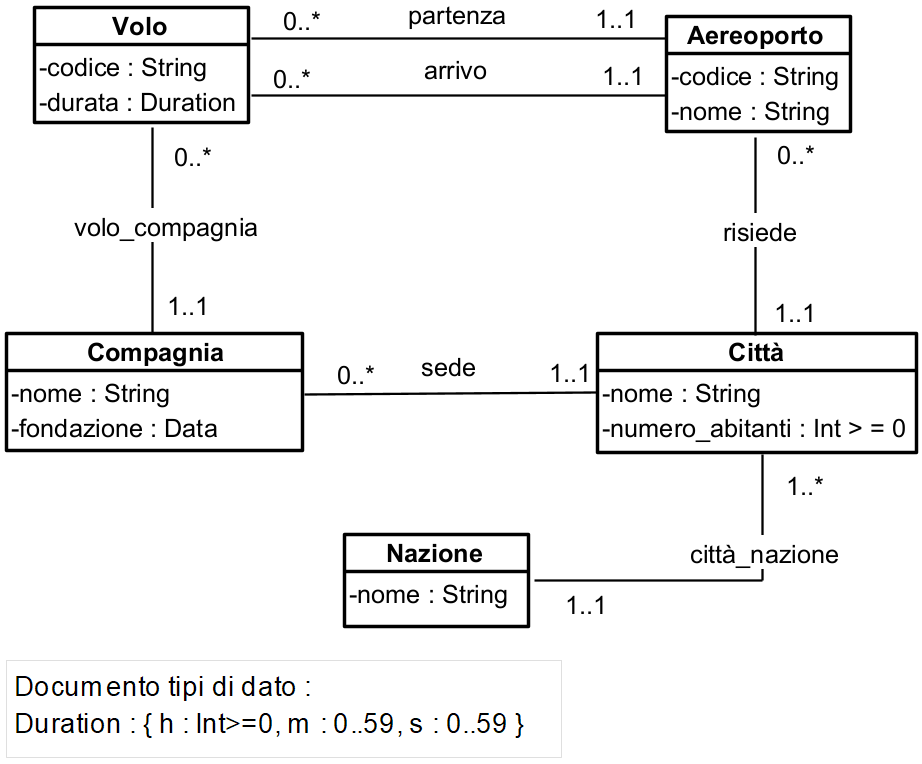
\includegraphics[width=\textwidth]{images/UML.png}


\end{document}

